\section{范数}
\label{sec:nspace-norms}

要判断两个函数整体上是否接近，先要给它们的差$f-g$规定一个“大小”，再用这个大小是否趋于零来判断近似是否成功。卷二已经用范数公理规定了向量的大小，本节把这套公理用到整个函数上。先说明函数范数的含义，再说明它给出的收敛与柯西列，最后说明无限维空间中不同范数之间可能无法互相控制。

\subsection{函数的范数}
\label{sec:nspace-function-norms}

函数的范数衡量的是整个函数的大小，而不是某一点处的函数值。要让不同的大小规则共享同一套推理，只要求它们满足几条共同的性质，这就是卷二的范数公理。

\begin{definition}[范数与赋范空间]
\label{def:nspace-norm}
设$V$是$\mathbb K$上的线性空间。映射$\lVert\cdot\rVert:V\to[0,\infty)$称为$V$上的\term{范数}（norm），若对所有$f,g\in V$与$c\in\mathbb K$：
\begin{enumerate}
 \item 正定性：$\lVert f\rVert=0$当且仅当$f=0$；
 \item 齐次性：$\lVert cf\rVert=\lvert c\rvert\,\lVert f\rVert$；
 \item 三角不等式：$\lVert f+g\rVert\leq\lVert f\rVert+\lVert g\rVert$。
\end{enumerate}
配备范数的线性空间$(V,\lVert\cdot\rVert)$称为\term{赋范空间}（normed space）。
\end{definition}

对函数而言，正定性中的“$f=0$”指$f$是零元素。在逐点运算的函数空间里，零元素是处处为零的函数，所以$\lVert f\rVert=0$必须迫使$f$在每一点都为零。齐次性说明把函数整体放大$c$倍，大小也放大$\lvert c\rvert$倍。三角不等式说明两段误差串联起来不超过各自之和，它是后面误差估计的基本工具。有限维范数的例子与性质，可参考\BookChapterRef{chap:normed-inner-product-spaces}{卷二第3章“赋范空间与内积空间”}。

\paragraph{两种整体大小}
在$C[0,1]$上，最常用的两种大小是
\[
 \lVert f\rVert_\infty=\max_{x\in[0,1]}\lvert f(x)\rvert,\qquad \lVert f\rVert_1=\int_0^1\lvert f(x)\rvert\,dx.
\]
前者看最坏的位置，后者看绝对值曲线下的总面积。对$h(x)=x-x^2$，$\lVert h\rVert_\infty=\tfrac14$，$\lVert h\rVert_1=\tfrac16$，这就是章首的两个数。两者都不是函数在某一点的值：$h(0)=0$，但$h$并不是零元素。

逐条核对公理。$\lVert\cdot\rVert_\infty$的齐次性和三角不等式在每个$x$处成立后取最大值即得；若最大值为$0$，则每点$\lvert f(x)\rvert=0$。$\lVert\cdot\rVert_1$的齐次性与三角不等式来自积分的线性与单调性。正定性需要连续：若$f$在某点$x_0$处$\lvert f(x_0)\rvert=a>0$，则在$x_0$附近的一个区间上$\lvert f\rvert>a/2$，积分为正。

\paragraph{有限性与正定性要逐个空间核验}
同一个公式放到别的函数集合上，公理可能不再成立。把$\int_0^1\lvert f\rvert$用于$[0,1]$上的有界黎曼可积函数，正定性失效：只在$x=\tfrac12$处取$1$、其余处取$0$的函数不是零函数，积分却为$0$。这样只满足齐次性与三角不等式、允许非零元素大小为零的函数称为\term{半范数}（seminorm）。

公式的值也可能是无穷。把$\max\lvert f\rvert$换成$\sup\lvert f\rvert$用于$\mathbb R$上的连续函数，$f(x)=x$的上确界为$+\infty$，不是实数。所以给一个函数集合配范数时，要分别核验三件事：集合对线性运算封闭，公式对集合中每个元素有限，正定性在这个集合上成立。第~\ref{sec:nspace-continuous-function-spaces}节到第~\ref{sec:nspace-linfty-space}节对各个具体空间逐一完成这些核验，其中积分范数的正定性要靠把几乎处处相等的函数看作同一个元素来恢复。

\subsection{范数与收敛}
\label{sec:nspace-norm-convergence}

范数给出距离$d(f,g)=\lVert f-g\rVert$。由三条公理可以直接验证距离公理，例如三角不等式$d(f,h)=\lVert(f-g)+(g-h)\rVert\leq d(f,g)+d(g,h)$。所以每个赋范空间都是度量空间，第~\ref{chap:metric-spaces}章关于点列收敛、柯西列、闭集和完备性的结论都可以直接使用。

\paragraph{依范数收敛与柯西列}
按这个距离，序列$(f_n)$收敛到$f$就是$\lVert f_n-f\rVert\to0$，称为\term{依范数收敛}（convergence in norm）。$(f_n)$是柯西列，就是对每个$\varepsilon>0$存在$N$，使$m,n\geq N$时$\lVert f_n-f_m\rVert<\varepsilon$。收敛列都是柯西列；反过来是否成立取决于空间，这是下一节的问题。

范数的选择决定了收敛控制什么。在$C[0,1]$上，$\lVert f_n-f\rVert_\infty\to0$说明对每个$\varepsilon>0$，从某个$N$起，所有输入处的误差同时不超过$\varepsilon$，这正是一致收敛。$\lVert f_n-f\rVert_1\to0$只说明误差曲线下的面积趋于零，允许在越来越窄的区间上保留较大的误差。由$\lVert h\rVert_1\leq\lVert h\rVert_\infty$，一致收敛推出积分误差收敛；下一小节将说明反过来不成立。

\paragraph{等价范数}
若同一空间上的两个范数能互相控制，它们给出的收敛判断就完全一致。

\begin{definition}[等价范数]
\label{def:nspace-equivalent-norms}
线性空间$V$上的两个范数$N_1,N_2$称为\term{等价范数}（equivalent norms），若存在常数$0<c\leq C$，使对所有$f\in V$，
\[
 c\,N_1(f)\leq N_2(f)\leq C\,N_1(f).
\]
\end{definition}

对$h=f_n-f$使用右边的不等式，$N_1(f_n-f)\to0$推出$N_2(f_n-f)\to0$；左边的不等式给出反方向。对$h=f_n-f_m$使用同样的不等式，两个范数下的柯西列也相同。所以等价范数给出相同的收敛序列、相同的极限和相同的柯西列，完备性也随之相同。关键是常数$c,C$与$f$无关。

有限维空间中，任意两个范数都等价，卷二已经证明了这一点。因此有限维空间的收敛与完备性不依赖范数的选择，只有误差的具体数值与常数随范数改变。卷二的证明用到有限维单位球面的紧性，上一章说明这一性质在无限维中失效，所以无限维空间中的两个范数是否等价，需要另作判断。

\subsection{范数不等价}
\label{sec:nspace-inequivalent-norms}

下面先从一般的无限维赋范空间出发，构造一个与原范数不等价的新范数，再在$C[0,1]$上给出一对具体的不等价范数。

\paragraph{用代数基构造}
设$(X,N_1)$是无限维赋范空间，$\{e_n\}_{n\geq1}$是第~\ref{chap:functions-as-vectors}章用Riesz引理构造的单位列：$N_1(e_n)=1$，且$\{e_n\}$线性无关。用选择公理可以把这个线性无关族扩充为$X$的一组代数基$B\supseteq\{e_n\}$，这里不给出证明。每个$x\in X$都唯一地写成$B$中有限个元素的组合。

在基上规定$Te_n=e_n/n$，对其余的$b\in B$规定$Tb=b$，再线性延拓：对$x=\sum_{b}c_bb$（有限和），令$Tx=\sum_bc_b\lambda_bb$，其中$\lambda_{e_n}=1/n$，其余$\lambda_b=1$。表示唯一，所以$T$是定义合理的线性映射。$T$还是单射：若$Tx=0$，由表示的唯一性，每个$c_b\lambda_b=0$，而$\lambda_b\neq0$，故每个$c_b=0$。

令$N_2(x)=N_1(Tx)$。它是范数：齐次性与三角不等式由$T$的线性和$N_1$的相应性质得到，例如$N_2(x+y)=N_1(Tx+Ty)\leq N_2(x)+N_2(y)$；若$N_2(x)=0$，则$Tx=0$，由单射得$x=0$。但
\[
 N_1(e_n)=1,\qquad N_2(e_n)=N_1(e_n/n)=\frac1n.
\]
若存在$c>0$使$cN_1\leq N_2$，取$x=e_n$得$c\leq1/n$对所有$n$成立，矛盾。所以$N_1$与$N_2$不等价：序列$e_n$在$N_2$下趋于零，在$N_1$下却始终与零相距$1$。

这个构造说明，每个无限维赋范空间上都存在与原范数不等价的范数。它是纯粹的存在性论证：代数基无法具体写出，$N_2$也就无法具体计算。

\paragraph{连续函数上的一对具体范数}
在$C[0,1]$上，$\lVert\cdot\rVert_\infty$与$\lVert\cdot\rVert_1$就不等价。一个方向的控制成立：$\lvert f(x)\rvert\leq\lVert f\rVert_\infty$对每个$x$成立，在$[0,1]$上积分得$\lVert f\rVert_1\leq\lVert f\rVert_\infty$。另一个方向没有常数：取$f_n(x)=x^n$，
\[
 \lVert x^n\rVert_\infty=1,\qquad \lVert x^n\rVert_1=\int_0^1x^n\,dx=\frac1{n+1}\to0.
\]
若$\lVert f\rVert_\infty\leq C\lVert f\rVert_1$，则$1\leq C/(n+1)$对所有$n$成立，矛盾。

图~\ref{fig:nspace-xn-norms}显示了这一差别的来源。$x^n$只在靠近$1$的越来越窄的区间上取较大的值，积分看到的是这段区间的面积，最大值看到的是峰顶。同一列函数在积分范数下趋于零函数，在最大值范数下与零函数的距离始终为$1$。图中的平方积分大小$\lVert x^n\rVert_2=(2n+1)^{-1/2}$在第~\ref{sec:nspace-lp-spaces}节正式定义。

\begin{figure}[!htb]
  \centering
  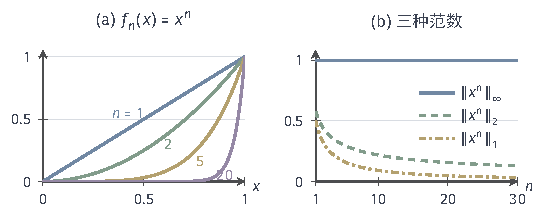
\includegraphics[width=92.3mm]{figures/02-abstract-mathematics/03-function-spaces/tikz/c1-xn-norms/figure.pdf}
  \caption{$x^n$在$[0,1]$上的三种大小。(a)$n=1,2,5,20$时的曲线，较大的函数值集中到右端越来越窄的区间上。(b)三种大小随$n$的变化：$\lVert x^n\rVert_\infty=1$保持不变，$\lVert x^n\rVert_2=(2n+1)^{-1/2}$与$\lVert x^n\rVert_1=(n+1)^{-1}$趋于零。}
  \label{fig:nspace-xn-norms}
\end{figure}

\paragraph{与有限维的对照}
卷二的结论是“有限维空间中任意两个范数都等价”。它在无限维中的否定是“存在不等价的范数”，而不是“任意两个范数都不等价”。例如$\lVert\cdot\rVert_\infty$与$2\lVert\cdot\rVert_\infty$在任何空间上都等价，常数为$c=C=2$。

因此在无限维空间中谈论收敛，必须同时说明用哪个范数。说“$x^n$在$C[0,1]$中收敛到$0$”是不完整的陈述：在$\lVert\cdot\rVert_1$下它成立，在$\lVert\cdot\rVert_\infty$下它不成立。后面各节始终把空间与范数一起给出。
